% Vortex Lattice Method (V.L.M.) -- Aerodynamic Characterization and Stall Optimization
% Revised edition. Build from the repository root with:  make report
\documentclass[11pt,letterpaper]{article}

\usepackage[T1]{fontenc}
\usepackage[utf8]{inputenc}
\usepackage{mathptmx}
\renewcommand{\ttdefault}{pcr}
\usepackage[margin=2.5cm,headheight=28pt]{geometry}
\usepackage{amsmath}
\usepackage{graphicx}
\usepackage{booktabs}
\usepackage{float}
\usepackage[font=small,labelfont=bf]{caption}
\usepackage{xcolor}
\usepackage{fancyhdr}
\usepackage{titlesec}
\usepackage{microtype}
\usepackage[hidelinks]{hyperref}
\usepackage[capitalise,noabbrev]{cleveref}

\graphicspath{{figures/}{logos/}}
\definecolor{upm}{RGB}{0,62,124}

\hypersetup{
  pdftitle={Vortex Lattice Method (V.L.M.): Aerodynamic Characterization and Stall Optimization},
  pdfauthor={Lucas García Franco, Carlos Pesquero Cañizares},
  pdfkeywords={vortex lattice method, wing aerodynamics, stall, XFLR5},
}

\titleformat{\section}{\Large\bfseries\color{upm}}{\thesection.}{0.6em}{}
\titleformat{\subsection}{\large\bfseries\color{upm}}{\thesubsection.}{0.6em}{}

\pagestyle{fancy}
\fancyhf{}
\fancyhead[L]{
\includegraphics[height=20pt]{upm}}
\fancyhead[R]{
\includegraphics[height=22pt]{etsiae}}
\fancyfoot[R]{\thepage}
\renewcommand{\headrulewidth}{0pt}

\newcommand{\repo}{\url{https://github.com/CPesquero/vlm-wing-aerodynamics}}
\newcommand{\dd}{\mathrm{d}}

\begin{document}

% ---------------------------------------------------------------- title page
\begin{titlepage}
  \centering
  \vspace*{3cm}
  {\fontsize{30}{36}\selectfont\bfseries Vortex Lattice Method\\[4pt] (V.L.M.)\par}
  \vspace{0.8cm}
  {\Large\bfseries Aerodynamic Characterization and Stall Optimization\par}
  \vspace{2.5cm}
  {\large García Franco, Lucas\\[6pt] Pesquero Cañizares, Carlos\par}
  \vspace{0.6cm}
  {\normalsize Universidad Politécnica de Madrid, ETSIAE\par}
  \vfill
  
\includegraphics[height=2.2cm]{upm}\hspace{1.5cm}
\includegraphics[height=2.4cm]{etsiae}\par
  \vspace{1cm}
  {\small Revised edition, October 2026. Code: \repo\par}
\end{titlepage}

\tableofcontents
\clearpage

% ---------------------------------------------------------------- 1
\section{Objectives of the Project}
The objectives of this project are the following:
\begin{itemize}
  \item Apply the vortex lattice method to determine the aerodynamic characteristics of a wing.
  \item Redesign the wing so that its stall starts near the root.
\end{itemize}

% ---------------------------------------------------------------- 2
\section{Baseline Data}
The baseline airfoil is the NACA 3217, which has, relative to the chord, a maximum camber $f$ of
3\,\%, located at $x_f = 0.20\,c$, and a maximum thickness $t$ of 17\,\% (\cref{fig:airfoil}).

\begin{figure}[H]
  \centering
  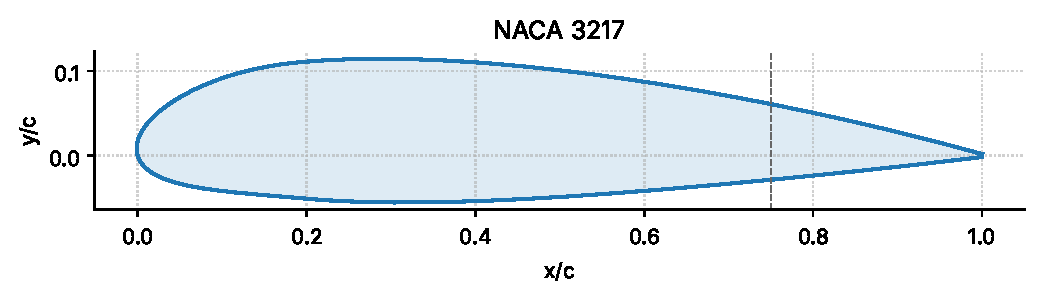
\includegraphics[width=0.8\linewidth]{airfoil}
  \caption{NACA 3217 airfoil. The dashed line marks the control point at $x/c = 0.75$.}
  \label{fig:airfoil}
\end{figure}

The wing parameters follow from the assignment values $W = 9$, $X = 3$, $Y = 5$, $Z = 5$, and are
listed in \cref{tab:baseline}.

\begin{table}[H]
  \centering
  \begin{tabular}{lc}
    \toprule
    Geometric parameter & Value \\
    \midrule
    Wing area ($S_w$) & 1\,m$^2$ \\
    Aspect ratio ($A$) & 15 \\
    Taper ratio ($\lambda$) & 0.65 \\
    Quarter-chord sweep ($\Lambda_{1/4}$) & 12$^\circ$ \\
    Geometric twist at the tip ($\varepsilon$), linear washout & $-5^\circ$ \\
    Chordwise panels ($N_x$) & 1 \\
    Spanwise panels per semispan ($N_y$) & 10 \\
    \bottomrule
  \end{tabular}
  \caption{Geometric parameters of the wing.}
  \label{tab:baseline}
\end{table}

\subsection{Wing Representation}
\Cref{fig:planform} shows the planform and the lattice: one horseshoe vortex per panel, bound on the
quarter-chord line, with its control point at three quarters of the local chord.

\begin{figure}[H]
  \centering
  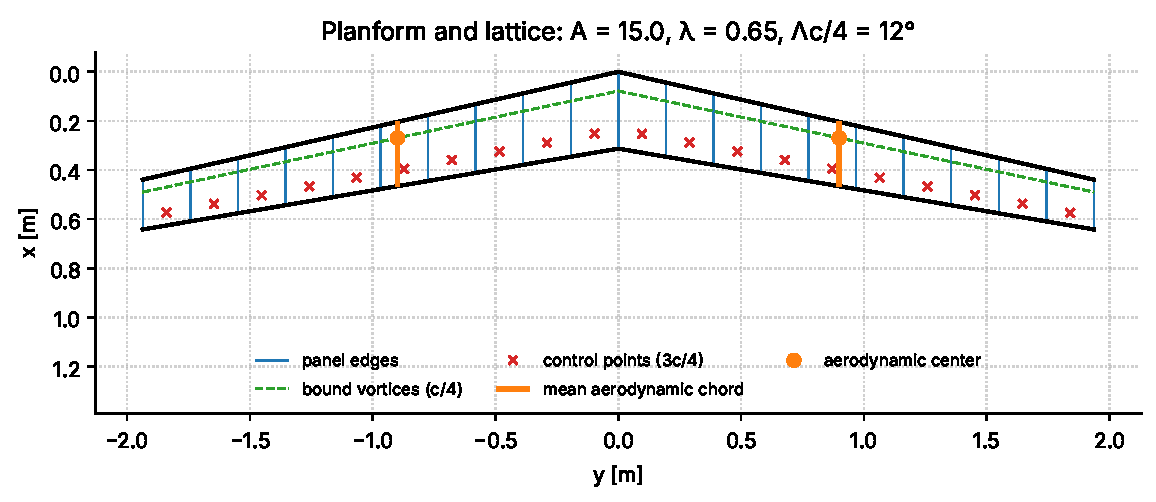
\includegraphics[width=\linewidth]{planform}
  \caption{Wing planform, vortex lattice, mean aerodynamic chord and aerodynamic center.}
  \label{fig:planform}
\end{figure}

% ---------------------------------------------------------------- 3
\section{Calculation of Geometric Parameters}
From the data of the statement, the following parameters are obtained~\cite{gandia}.

\begin{itemize}
  \item \textbf{Camber-line slope at the control point.} For a NACA four-digit airfoil, aft of the
  maximum camber ($x/c = 0.75 > x_f = 0.20$), and with $f = 0.03$, $x_f = 0.20$:
  \begin{equation}
    \frac{\dd z_c}{\dd x} = \frac{2f}{(1-x_f)^2}\left(x_f - \frac{x}{c}\right)
    \label{eq:camber}
  \end{equation}
  \item \textbf{Wingspan:}
  \begin{equation}
    A = \frac{b^2}{S}
  \end{equation}
  \item \textbf{Root chord}, solving
  \begin{equation}
    S = \frac{b}{2}\, c_0 \,(1+\lambda)
  \end{equation}
  \item \textbf{Tip chord:}
  \begin{equation}
    c_t = \lambda\, c_0
  \end{equation}
  \item \textbf{Geometric mean chord:}
  \begin{equation}
    c_{gm} = \frac{c_0 + c_t}{2}
  \end{equation}
  \item \textbf{Mean aerodynamic chord:}
  \begin{equation}
    c_{am} = \frac{2}{3}\, c_0\, \frac{1+\lambda+\lambda^2}{1+\lambda}
  \end{equation}
  \item \textbf{Aerodynamic center of the wing.} The leading-edge sweep follows from the
  quarter-chord sweep and the taper,
  \begin{equation}
    \tan\Lambda_{LE} = \tan\Lambda_{1/4} + \frac{c_0}{2b}\,(1-\lambda)
    \label{eq:sweep}
  \end{equation}
  and the aerodynamic center lies at a quarter of the mean aerodynamic chord, at its spanwise station:
  \begin{align}
    y_{ca} &= \frac{b}{6}\,\frac{1+2\lambda}{1+\lambda} \\
    x_{ca} &= y_{ca}\tan\Lambda_{LE} + 0.25\, c_{am}
  \end{align}
\end{itemize}

The resulting values are given in \cref{tab:geometry}.

\begin{table}[H]
  \centering
  \begin{tabular}{lc}
    \toprule
    Geometric parameter & Value \\
    \midrule
    Camber-line slope at $x = 3c/4$ & $-0.0516$ \\
    Wingspan ($b$) & 3.873\,m \\
    Root chord ($c_0$) & 0.313\,m \\
    Tip chord ($c_t$) & 0.203\,m \\
    Geometric mean chord ($c_{gm}$) & 0.258\,m \\
    Mean aerodynamic chord ($c_{am}$) & 0.262\,m \\
    Leading-edge sweep ($\Lambda_{LE}$) & 12.78$^\circ$ \\
    Aerodynamic center ($x_{ca}$, $y_{ca}$) & (0.2694, 0.8994)\,m \\
    \bottomrule
  \end{tabular}
  \caption{Derived wing parameters.}
  \label{tab:geometry}
\end{table}

% ---------------------------------------------------------------- 4
\section{Local Lift Coefficients}
For each angle of attack $\alpha$, the spanwise circulation $\{\Gamma_j\}$ is found by solving the
linear system
\begin{equation}
  [a_{ij}]\left\{\frac{\Gamma_j}{U_\infty}\right\} = -\{b_i\},
  \qquad
  b_i = \alpha + \varepsilon(y_i) - \left(\frac{\dd z_c}{\dd x}\right)_{3c/4}
  \label{eq:system}
\end{equation}
where $[a_{ij}]$ is the influence matrix of the horseshoe-vortex lattice (normal velocity induced at
control point $i$ by a unit vortex on panel $j$, from the Biot--Savart law~\cite{bertin}), and $b_i$
expresses the no-penetration condition at each control point, including the local geometric twist
$\varepsilon(y_i)$ and the camber-line slope of \cref{eq:camber}.

The Kutta--Joukowski theorem then gives the sectional lift coefficient:
\begin{equation}
  c_l(y_i) = \frac{2\,\Gamma(y_i)}{U_\infty\, c(y_i)}
\end{equation}

\Cref{tab:cl} lists the results for the right half-wing (the wing is symmetric) and
\cref{fig:cl} shows the whole span.

\begin{table}[H]
  \centering
  \begin{tabular}{ccrrrrr}
    \toprule
    Panel & $y$ [m] & $c_l(-12^\circ)$ & $c_l(-6^\circ)$ & $c_l(0^\circ)$ & $c_l(6^\circ)$ & $c_l(12^\circ)$ \\
    \midrule
    1  & 0.097 & $-0.881$ & $-0.342$ & $0.198$ & 0.737 & 1.277 \\
    2  & 0.290 & $-0.939$ & $-0.379$ & $0.181$ & 0.741 & 1.302 \\
    3  & 0.484 & $-0.993$ & $-0.420$ & $0.154$ & 0.727 & 1.300 \\
    4  & 0.678 & $-1.044$ & $-0.462$ & $0.119$ & 0.701 & 1.283 \\
    5  & 0.871 & $-1.092$ & $-0.505$ & $0.081$ & 0.667 & 1.254 \\
    6  & 1.065 & $-1.135$ & $-0.547$ & $0.040$ & 0.628 & 1.216 \\
    7  & 1.259 & $-1.169$ & $-0.585$ & $-0.001$ & 0.583 & 1.167 \\
    8  & 1.452 & $-1.186$ & $-0.614$ & $-0.041$ & 0.531 & 1.103 \\
    9  & 1.646 & $-1.161$ & $-0.619$ & $-0.077$ & 0.465 & 1.007 \\
    10 & 1.840 & $-0.997$ & $-0.546$ & $-0.094$ & 0.358 & 0.810 \\
    \bottomrule
  \end{tabular}
  \caption{Sectional lift coefficient of each panel (right half-wing) for each angle of attack.}
  \label{tab:cl}
\end{table}

\begin{figure}[H]
  \centering
  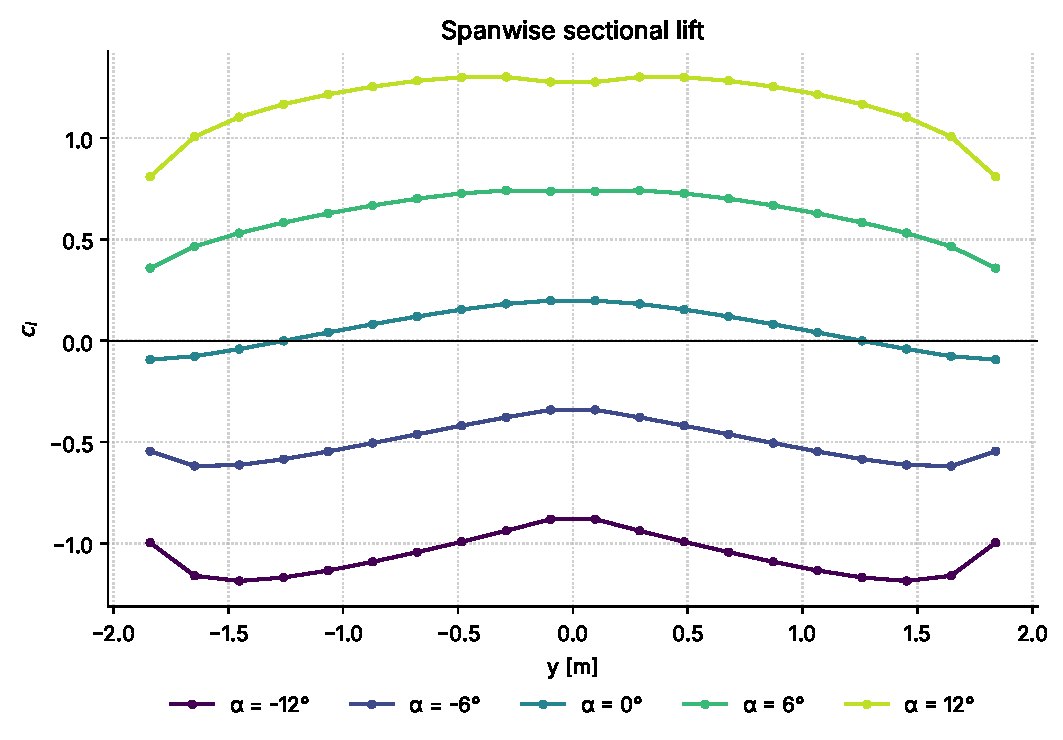
\includegraphics[width=0.85\linewidth]{lift_distribution}
  \caption{Spanwise sectional lift distribution. The dip at the root is a sweep effect.}
  \label{fig:cl}
\end{figure}

% ---------------------------------------------------------------- 5
\section{Global Lift Coefficient}
The global lift coefficient is obtained by integrating the sectional lift along the span:
\begin{equation}
  C_L = \frac{1}{S}\sum_{i=1}^{N} c_{l,i}\, c_i\, \Delta y_i
\end{equation}

The model is linear (attached, inviscid flow), so $C_L(\alpha)$ is a straight line. Its slope and its
value at $\alpha = 0$ are obtained by a least-squares fit through the five angles of attack,
\begin{equation}
  C_L = C_{L,\alpha=0} + C_{L\alpha}\,\alpha
\end{equation}
and the zero-lift angle follows as
\begin{equation}
  \alpha_{L=0} = -\frac{C_{L,\alpha=0}}{C_{L\alpha}}
\end{equation}
which measures the combined effect of camber and twist on the complete wing.

\begin{table}[H]
  \centering
  \begin{tabular}{ccc}
    \toprule
    $C_{L\alpha}$ & $C_{L,\alpha=0}$ & $\alpha_{L=0}$ \\
    \midrule
    0.0932\,deg$^{-1}$ (5.342\,rad$^{-1}$) & 0.068 & $-0.733^\circ$ \\
    \bottomrule
  \end{tabular}
  \caption{Lift-curve slope, lift at zero incidence and zero-lift angle.}
  \label{tab:CL}
\end{table}

\begin{figure}[H]
  \centering
  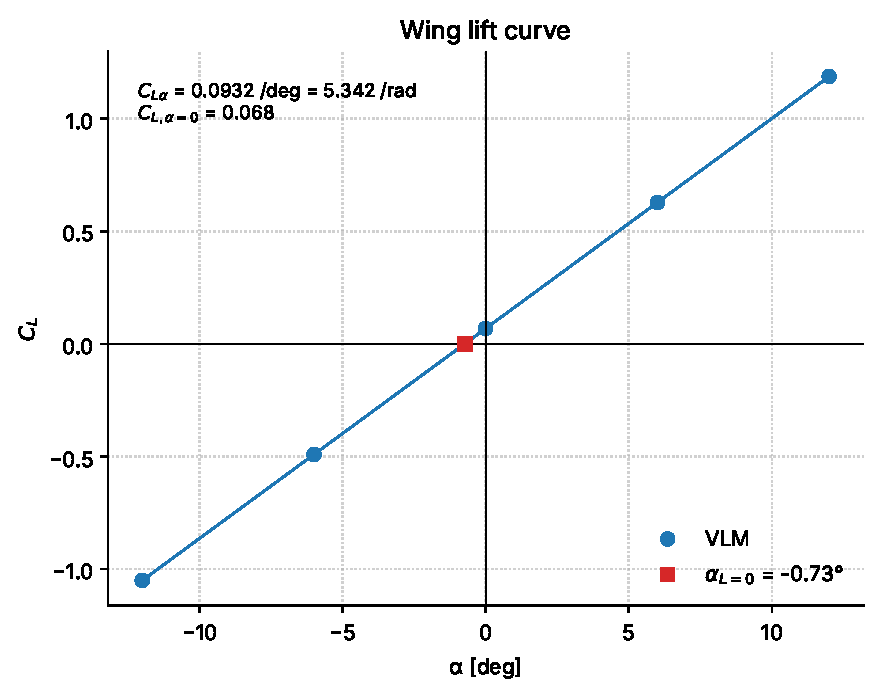
\includegraphics[width=0.62\linewidth]{lift_curve}
  \caption{Wing lift curve $C_L(\alpha)$.}
  \label{fig:CL}
\end{figure}

\Cref{fig:CL} shows the linear response with $C_{L,\alpha=0} = 0.068$: the camber of the airfoil
produces lift at zero incidence, partly offset by the washout of the tips.

% ---------------------------------------------------------------- 6
\section{Basic and Unit Additional Lift Distribution}
Because the problem is linear, the sectional lift can be split into a basic part, due to camber and
twist, and a unit additional part, due to the angle of attack and scaled by the global lift:
\begin{equation}
  c_l(y) = c_{l,b}(y) + c_{l,a}(y)\, C_L
\end{equation}

\begin{itemize}
  \item \textbf{Basic lift} $c_{l,b}$: the system of \cref{eq:system} is solved at the zero-lift angle.
  The global coefficient is zero, but twist and camber still produce a non-zero local load:
  \begin{equation}
    [a_{ij}]\left\{\frac{\Gamma_{b,j}}{U_\infty}\right\}
      = -\left(\alpha_{L=0} + \varepsilon(y_i) - \frac{\dd z_c}{\dd x}\right),
    \qquad
    c_{l,b} = \frac{2\,\Gamma_b}{U_\infty\, c}
  \end{equation}
  \item \textbf{Unit additional lift} $c_{l,a}$: twist and camber are removed, a uniform incidence is
  applied, and the result is normalized to $C_L = 1$:
  \begin{equation}
    c_{l,a} = \frac{c_{l,\text{planform}}(y)}{C_{L,\text{planform}}}
  \end{equation}
\end{itemize}

\begin{table}[H]
  \centering
  \begin{tabular}{cccc}
    \toprule
    Panel & $y$ [m] & $c_{l,b}$ & $c_{l,a}$ \\
    \midrule
    1  & 0.097 & 0.132 & 0.964 \\
    2  & 0.290 & 0.113 & 1.001 \\
    3  & 0.484 & 0.084 & 1.025 \\
    4  & 0.678 & 0.048 & 1.040 \\
    5  & 0.871 & 0.009 & 1.048 \\
    6  & 1.065 & $-0.031$ & 1.050 \\
    7  & 1.259 & $-0.072$ & 1.044 \\
    8  & 1.452 & $-0.111$ & 1.023 \\
    9  & 1.646 & $-0.143$ & 0.969 \\
    10 & 1.840 & $-0.149$ & 0.807 \\
    \bottomrule
  \end{tabular}
  \caption{Basic and unit additional lift coefficients (right half-wing).}
  \label{tab:basic}
\end{table}

\begin{figure}[H]
  \centering
  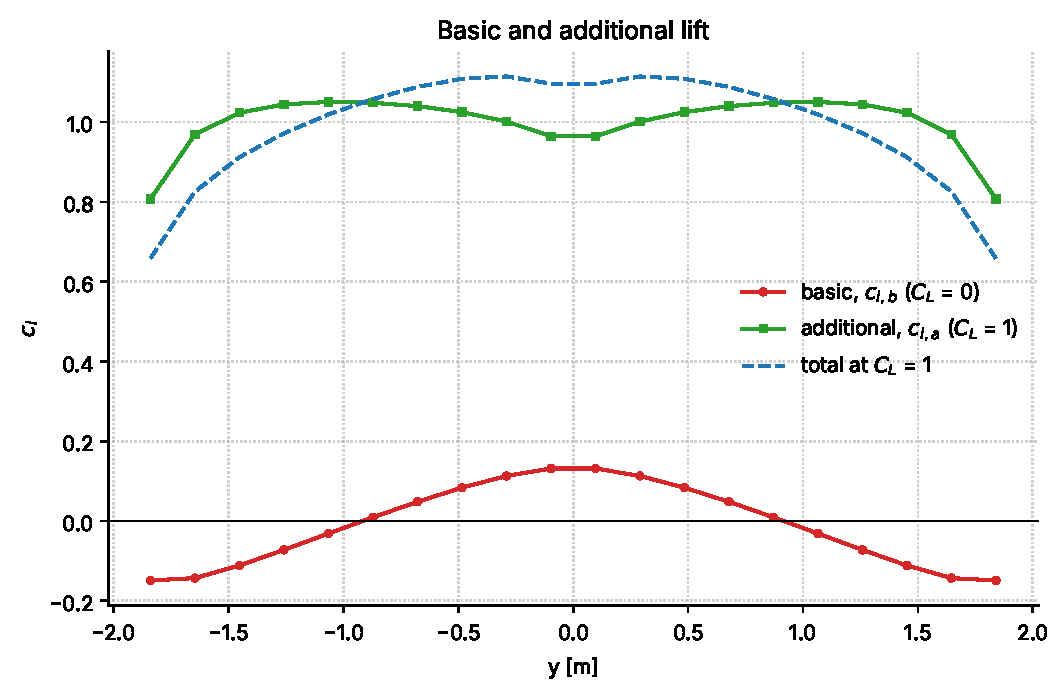
\includegraphics[width=0.85\linewidth]{basic_additional_lift}
  \caption{Basic and unit additional lift distributions.}
  \label{fig:basic}
\end{figure}

The basic load is positive inboard and negative at the tips: the washout unloads the tips. The
additional load is fairly flat over most of the span, with the root dip caused by sweep, and falls
off near the tips.

% ---------------------------------------------------------------- 7
\section{Induced Drag Coefficients}
The downwash produced by the trailing vortices is evaluated in the Trefftz plane, far downstream.
The influence matrix of the semi-infinite trailing legs is
\begin{equation}
  A^{T}_{ij} = \frac{1}{2\pi}\left(\frac{1}{y_i - y_{\text{left},j}} - \frac{1}{y_i - y_{\text{right},j}}\right)
\end{equation}
Multiplying it by the circulation vector gives the far-wake normal velocity $w_T$. The induced
angle at the wing is half of it,
\begin{equation}
  \alpha_i = \frac{w_T}{2\,U_\infty}
\end{equation}
and the local induced drag is the projection of the local lift onto the inclined flow:
\begin{equation}
  c_{di}(y) = c_l(y)\, \alpha_i(y)
\end{equation}
The global coefficient is obtained by integration over the span:
\begin{equation}
  C_{Di} = \frac{1}{S}\sum_{i=1}^{N} c_{di,i}\, c_i\, \Delta y_i
\end{equation}

\begin{table}[H]
  \centering
  \begin{tabular}{ccrrrrr}
    \toprule
    Panel & $y$ [m] & $c_{di}(-12^\circ)$ & $c_{di}(-6^\circ)$ & $c_{di}(0^\circ)$ & $c_{di}(6^\circ)$ & $c_{di}(12^\circ)$ \\
    \midrule
    1  & 0.097 & 0.0061 & $-0.0006$ & 0.0021 & 0.0143 & 0.0360 \\
    2  & 0.290 & 0.0114 & 0.0008 & 0.0014 & 0.0132 & 0.0362 \\
    3  & 0.484 & 0.0144 & 0.0020 & 0.0008 & 0.0108 & 0.0321 \\
    4  & 0.678 & 0.0170 & 0.0031 & 0.0003 & 0.0087 & 0.0281 \\
    5  & 0.871 & 0.0199 & 0.0044 & 0.0001 & 0.0069 & 0.0249 \\
    6  & 1.065 & 0.0235 & 0.0060 & 0.0000 & 0.0055 & 0.0226 \\
    7  & 1.259 & 0.0286 & 0.0080 & 0.0000 & 0.0046 & 0.0218 \\
    8  & 1.452 & 0.0363 & 0.0109 & 0.0002 & 0.0041 & 0.0227 \\
    9  & 1.646 & 0.0487 & 0.0154 & 0.0006 & 0.0044 & 0.0266 \\
    10 & 1.840 & 0.0657 & 0.0213 & 0.0012 & 0.0052 & 0.0335 \\
    \bottomrule
  \end{tabular}
  \caption{Local induced drag coefficient (right half-wing).}
  \label{tab:cdi}
\end{table}

\begin{table}[H]
  \centering
  \begin{tabular}{cccccc}
    \toprule
    $\alpha$ & $-12^\circ$ & $-6^\circ$ & $0^\circ$ & $6^\circ$ & $12^\circ$ \\
    \midrule
    $C_{Di}$ & 0.0251 & 0.0063 & 0.0007 & 0.0082 & 0.0288 \\
    \bottomrule
  \end{tabular}
  \caption{Global induced drag coefficient.}
  \label{tab:CDi}
\end{table}

\begin{figure}[H]
  \centering
  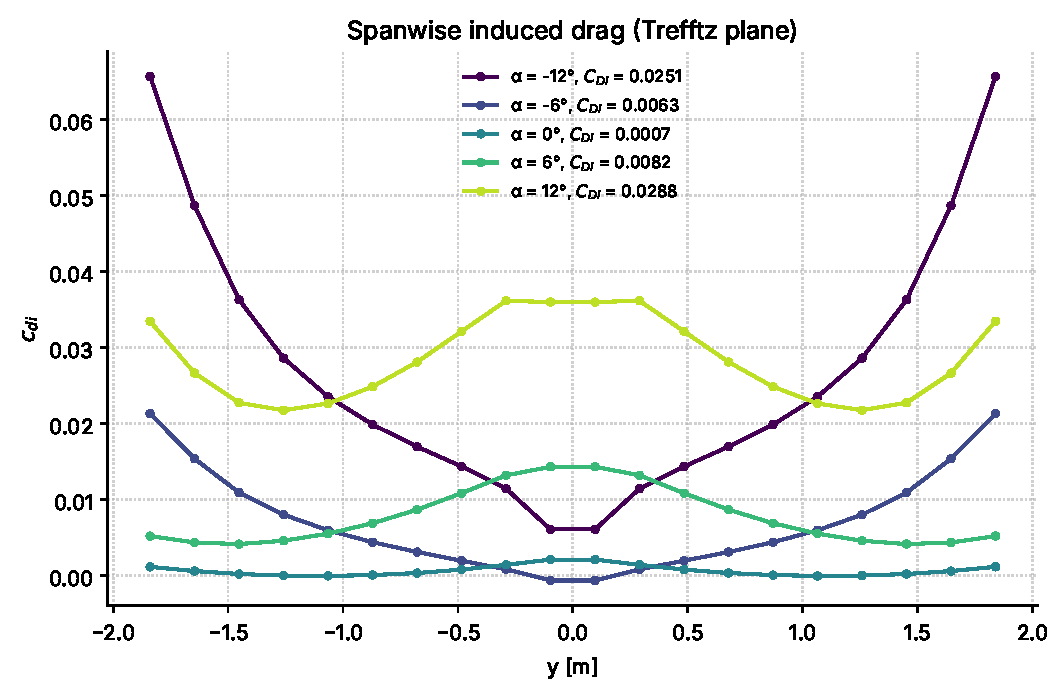
\includegraphics[width=0.85\linewidth]{induced_drag}
  \caption{Spanwise induced drag distribution.}
  \label{fig:cdi}
\end{figure}

Induced drag is smallest near zero incidence and grows with $|\alpha|$. At negative angles it
concentrates at the tips, where the washout adds to the negative load. The small negative local
values near the root at $-6^\circ$ are local upwash, not a net thrust: the global $C_{Di}$ is positive at
every angle.

% ---------------------------------------------------------------- 8
\section{Pitching Moment}
The pitching moment is computed about two reference points: the coordinate origin (root leading
edge) and the aerodynamic center of the wing, $x_{ca}$. In this one-chordwise-panel model the lift of
each panel acts on its quarter-chord line:
\begin{equation}
  x_{1/4}(y) = |y|\tan\Lambda_{LE} + 0.25\, c(y)
\end{equation}
The moment about the origin (nose-up positive, reference chord $c_{am}$) is
\begin{equation}
  C_{M,0y} = \frac{1}{S\, c_{am}}\sum_{i=1}^{N} \left(-c_{l,i}\, c_i\, x_{1/4,i}\, \Delta y_i\right)
\end{equation}
and it is transferred to the aerodynamic center with
\begin{equation}
  C_{M,ca} = C_{M,0y} + C_L\, \frac{x_{ca}}{c_{am}}
\end{equation}

\begin{table}[H]
  \centering
  \begin{tabular}{ccc}
    \toprule
    $\alpha$ & $C_{M,0y}$ & $C_{M,ca}$ \\
    \midrule
    $-12^\circ$ & 1.115 & 0.034 \\
    $-6^\circ$ & 0.545 & 0.040 \\
    $0^\circ$ & $-0.026$ & 0.045 \\
    $6^\circ$ & $-0.596$ & 0.050 \\
    $12^\circ$ & $-1.166$ & 0.055 \\
    \bottomrule
  \end{tabular}
  \caption{Pitching moment coefficients.}
  \label{tab:CM}
\end{table}

\begin{figure}[H]
  \centering
  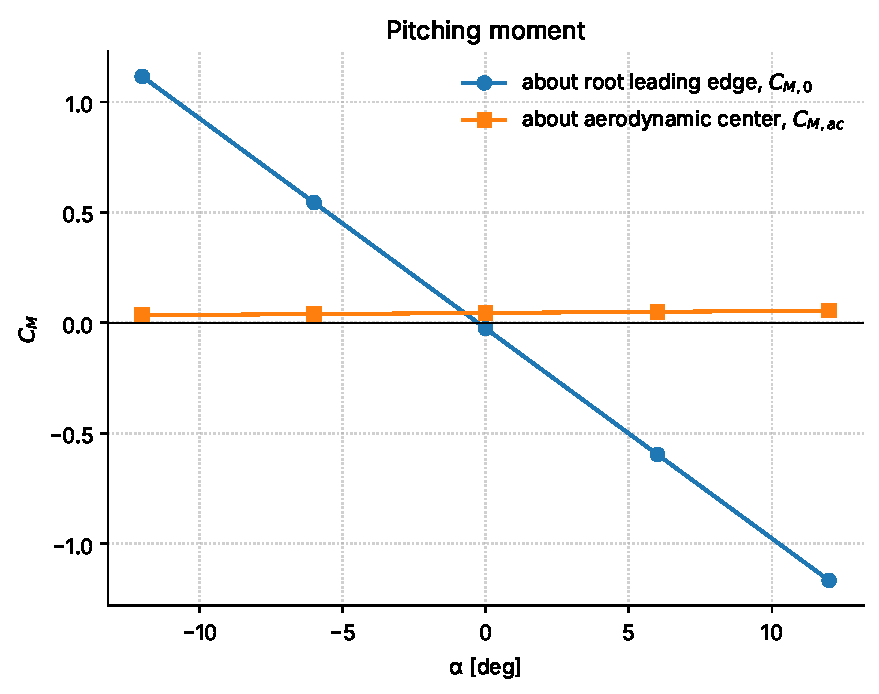
\includegraphics[width=0.62\linewidth]{pitching_moment}
  \caption{Pitching moment coefficients versus angle of attack.}
  \label{fig:CM}
\end{figure}

About the origin the moment varies strongly with $\alpha$. About the aerodynamic center it is small
and nearly constant: it drifts from 0.034 to 0.055 over the whole range, so $x_{ca}$ is correctly
located. The small drift, $\dd C_{M,ca}/\dd C_L \approx 0.009$, means that the exact aerodynamic center
of the lattice lies about 2.5\,mm ahead of the quarter-MAC estimate. The positive $C_{M,ca}$ comes from
the washout of the swept-back tips, which carry negative lift behind the aerodynamic center. With a
single chordwise panel all the load acts on the quarter-chord line, so the nose-down moment of the
cambered airfoil itself is not represented. Longitudinal stability itself cannot be assessed from these values alone: it requires
the center of gravity and the rest of the aircraft (fuselage, tail), which are outside this study.

% ---------------------------------------------------------------- 9
\section{Validation and Mesh Sensitivity}

\subsection{Comparison with XFLR5}
\Cref{fig:xflr5} compares the sectional lift with an XFLR5~\cite{xflr5} analysis exported at the
same 20 spanwise stations, so the comparison is point by point.

\begin{figure}[H]
  \centering
  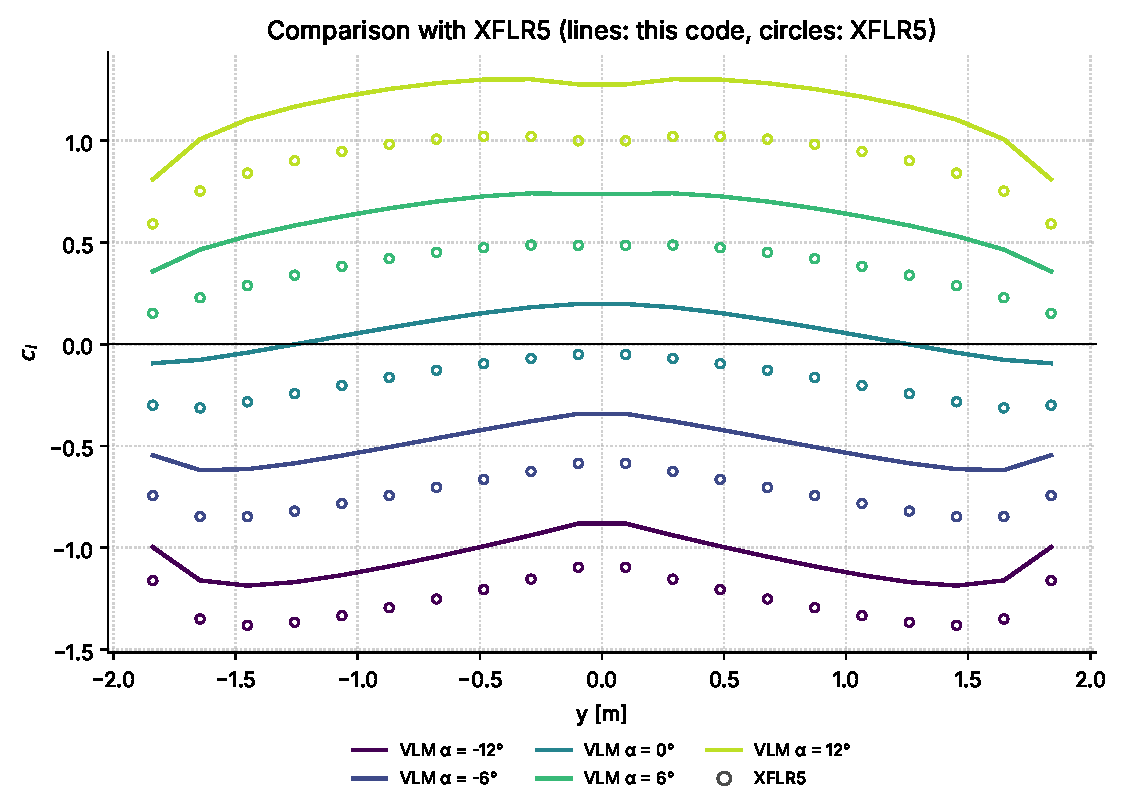
\includegraphics[width=0.9\linewidth]{xflr5_comparison}
  \caption{Sectional lift: this code (lines) and XFLR5 (circles) at the same stations.}
  \label{fig:xflr5}
\end{figure}

\begin{itemize}
  \item \textbf{Shape.} Both models give the same distribution shape, including the dip at the plane of
  symmetry caused by the sweep ($\Lambda_{1/4} = 12^\circ$).
  \item \textbf{Lift slope.} The spacing between curves agrees: integrating the XFLR5 data gives
  $C_{L\alpha} = 0.0909$\,deg$^{-1}$, within 2.6\,\% of the 0.0932\,deg$^{-1}$ of this code.
  \item \textbf{Absolute level.} There is a near-constant offset of 0.20 to 0.27 in $c_l$ between the two,
  so the zero-lift angles differ. A likely cause is the camber model: this code applies a single
  camber slope at $3c/4$ (\cref{eq:camber}), while XFLR5 panels the actual mean line.
\end{itemize}
The agreement therefore validates the slope and the shape of the distribution, not the absolute
lift at a given angle.

\subsection{Mesh sensitivity}
\Cref{tab:mesh,fig:mesh} show $C_L$ at $\alpha = 6^\circ$ as the number of spanwise panels (whole wing)
increases.

\begin{table}[H]
  \centering
  \begin{tabular}{ccc}
    \toprule
    Panels (whole wing) & $C_L$ & Solve time [ms] \\
    \midrule
    4   & 0.6394 & 0.2 \\
    10  & 0.6336 & 0.2 \\
    20  & 0.6277 & 0.2 \\
    40  & 0.6232 & 0.4 \\
    80  & 0.6207 & 1.1 \\
    120 & 0.6199 & 2.4 \\
    160 & 0.6194 & 4.4 \\
    320 & 0.6188 & 14.5 \\
    \bottomrule
  \end{tabular}
  \caption{Mesh sensitivity at $\alpha = 6^\circ$. Times are machine-dependent.}
  \label{tab:mesh}
\end{table}

\begin{figure}[H]
  \centering
  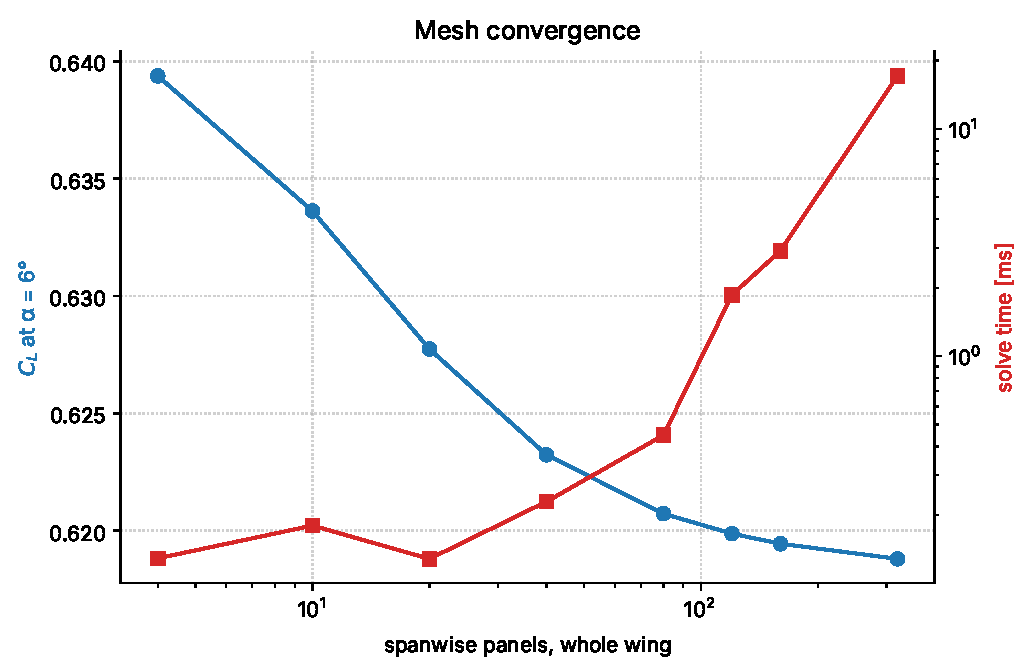
\includegraphics[width=0.72\linewidth]{mesh_convergence}
  \caption{Convergence of $C_L$ and computational cost with the number of panels.}
  \label{fig:mesh}
\end{figure}

$C_L$ decreases monotonically and changes by less than 0.5\,\% from 80 panels onward, which is the
recommended resolution for accurate results. The cost grows polynomially with the number of panels
$N$ (assembly of the $N\times N$ influence matrix and a dense solve), not exponentially, and stays in
milliseconds even at 320 panels. The results of \cref{tab:cl,tab:CL,tab:basic,tab:cdi,tab:CDi,tab:CM}
use the 20 panels of the statement; at 80 panels $C_L$ is about 1.1\,\% lower.

% ---------------------------------------------------------------- 10
\section{Optimization of Stall Characteristics}
The objective of this section is to redesign the baseline wing so that the loss of lift begins
within 40\,\% of the semispan (with $y = 0$ at the root) and the sectional lift falls off outboard of
that point with a gradient of at least $\dd c_l/\dd y = -0.2$\,m$^{-1}$.

\textbf{Methodological note.} Under the hypothesis of a linear potential regime, stall onset is taken
as the station of maximum sectional lift $c_l(y)$ at a high angle of attack ($\alpha = 15^\circ$). It is
assumed that the airfoil has a maximum lift coefficient $c_{l,\max}$ that is uniform along the span, so
the lift peak marks the section where the boundary layer would separate first in real flight. This is
a modelling assumption: the VLM itself does not represent separation.

\textbf{Baseline.} At $\alpha = 15^\circ$ the baseline lift peak is already at 25\,\% of the semispan, but
the gradient outboard of it is only $-0.069$\,m$^{-1}$, so the objective is not met.

\textbf{Search.} The code evaluates every combination of aspect ratio (15 to 4), quarter-chord sweep
(0 to 24$^\circ$), taper ratio (0.1 to 1), tip twist (0 to $-9^\circ$) and airfoil (NACA 0012, 2412,
3217, 4417), about 440\,000 designs. The wing area is held at 1\,m$^2$ for every design, so the aspect
ratio is exact. The feasible designs are ranked by their normalized distance from the baseline
planform:
\begin{equation}
  J = \sqrt{\left(\frac{\Delta A}{A_0}\right)^2 + \left(\frac{\Delta\Lambda_{1/4}}{\Lambda_{1/4,0}}\right)^2
      + \left(\frac{\Delta\lambda}{\lambda_0}\right)^2 + \left(\frac{\Delta\varepsilon}{\varepsilon_0}\right)^2}
\end{equation}
Of all the designs, 1\,529 meet both requirements. The five closest to the baseline are listed in
\cref{tab:opt}.

\begin{table}[H]
  \centering
  \begin{tabular}{lcccccccc}
    \toprule
    & Airfoil & $A$ & $\Lambda_{1/4}$ & $\lambda$ & $\varepsilon$ & Peak at & $\dd c_l/\dd y$ [m$^{-1}$] & $J$ \\
    \midrule
    Baseline & 3217 & 15.0 & 12$^\circ$ & 0.65 & $-5^\circ$ & 25\,\% & $-0.069$ & -- \\
    \midrule
    1 & 0012 & 11.5 & 3$^\circ$ & 1.00 & $-8^\circ$ & 5\,\% & $-0.200$ & 1.127 \\
    2 & 0012 & 13.5 & 5$^\circ$ & 1.00 & $-9^\circ$ & 5\,\% & $-0.200$ & 1.133 \\
    3 & 0012 & 11.0 & 3$^\circ$ & 1.00 & $-8^\circ$ & 5\,\% & $-0.201$ & 1.135 \\
    4 & 0012 & 13.0 & 5$^\circ$ & 1.00 & $-9^\circ$ & 5\,\% & $-0.201$ & 1.137 \\
    5 & 0012 & 12.5 & 5$^\circ$ & 1.00 & $-9^\circ$ & 5\,\% & $-0.201$ & 1.141 \\
    \bottomrule
  \end{tabular}
  \caption{Baseline and the five feasible designs closest to it ($\alpha = 15^\circ$, 20 panels).}
  \label{tab:opt}
\end{table}

The best design is a NACA 0012 wing with $A = 11.5$, $\Lambda_{1/4} = 3^\circ$, $\lambda = 1.0$ and
$\varepsilon = -8^\circ$ (span 3.391\,m, constant chord 0.295\,m). Its lift peak is at the innermost
panel (5\,\% of the semispan) and the gradient is $\dd c_l/\dd y = -0.200$\,m$^{-1}$
(\cref{fig:opt,fig:optplan}).

\begin{figure}[H]
  \centering
  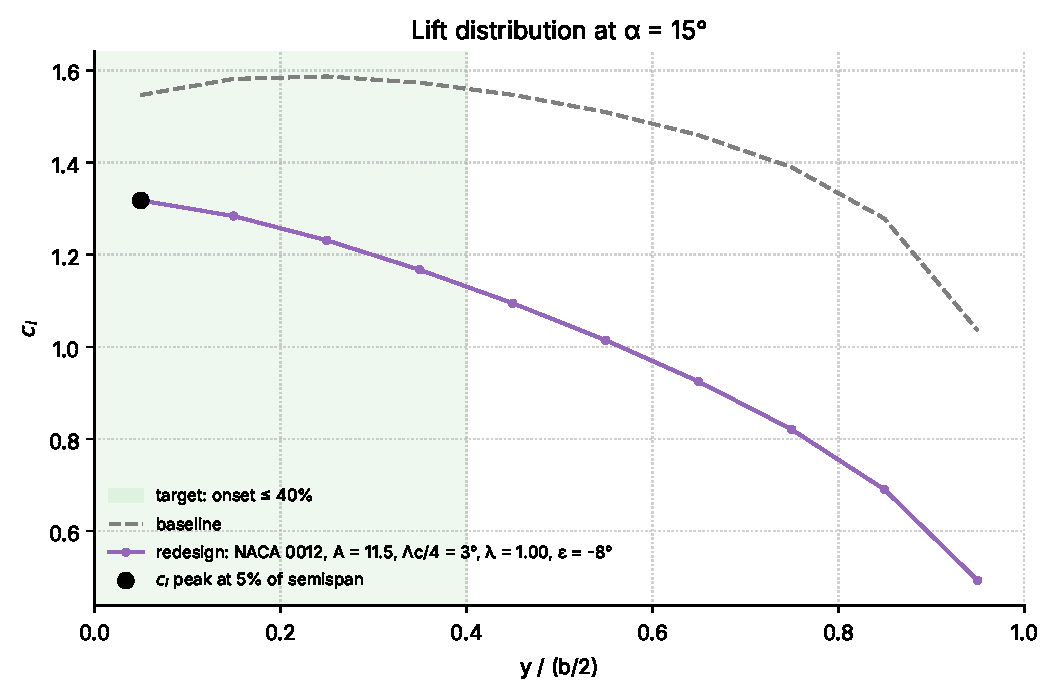
\includegraphics[width=0.85\linewidth]{optimized_lift}
  \caption{Lift distribution at $\alpha = 15^\circ$ of the baseline and the redesigned wing, with the stall point.}
  \label{fig:opt}
\end{figure}

\begin{figure}[H]
  \centering
  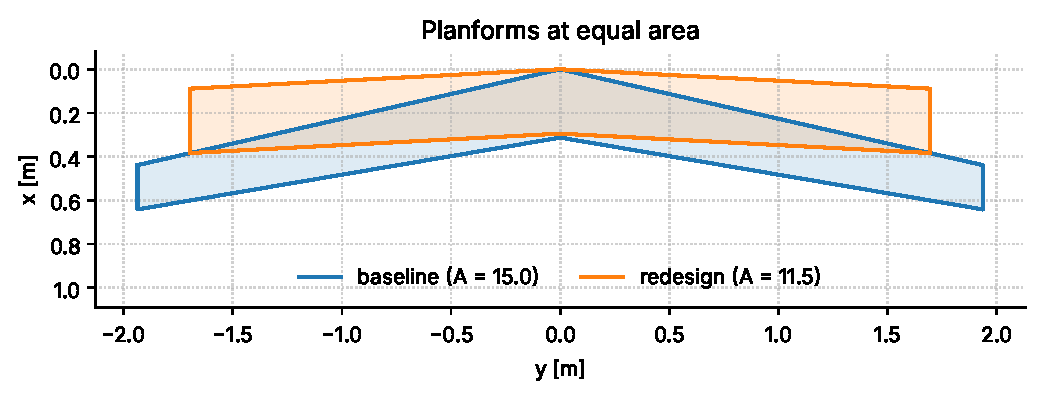
\includegraphics[width=0.8\linewidth]{planform_comparison}
  \caption{Baseline and redesigned planforms at equal area.}
  \label{fig:optplan}
\end{figure}

\textbf{Role of each parameter.}
\begin{itemize}
  \item \textbf{Twist} is the most effective parameter. More washout reduces the local angle of attack
  at the tips and moves the lift peak towards the root. The penalty appears in cruise: the redesigned
  wing has a sectional lift of $-0.39$ at the tip at $\alpha = 0$, and the departure from the optimum load
  raises induced drag and bending loads.
  \item \textbf{Sweep} moves load outboard, so the search reduces it from 12$^\circ$ to 3$^\circ$.
  \item \textbf{Taper ratio.} A rectangular wing ($\lambda = 1$) has more chord at the tips and carries
  relatively less load there, which also favours root stall. It moves away from the elliptical
  distribution and loses efficiency.
  \item \textbf{Aspect ratio} has a secondary effect on where the stall starts, but a lower aspect ratio
  raises induced drag in cruise.
  \item \textbf{Airfoil.} In this model the airfoil enters only through its camber slope, which shifts
  the whole distribution without changing its shape. All top designs use the symmetric NACA 0012
  because less camber helps meet the gradient threshold at $15^\circ$. The real effect of an airfoil
  change on stall, through $c_{l,\max}$ and thickness, is not captured; in practice a thicker root
  section would be chosen to make the root stall gently and give warning.
\end{itemize}

\textbf{Cost of the redesign.} At a cruise lift coefficient $C_L = 0.5$, the redesigned wing needs
$\alpha = 9.3^\circ$ instead of $4.6^\circ$, and its induced drag rises from $C_{Di} = 0.0053$ to
$0.0072$ (+36\,\%; span efficiency 0.96 versus 1.00).

% ---------------------------------------------------------------- 11
\section{Conclusions}
A numerical model based on the vortex lattice method has been developed and applied to the
aerodynamic characterization of a swept, tapered and twisted wing. The geometric parameters were
defined, including the mean aerodynamic chord and the location of the aerodynamic center. The
sectional and global lift were computed and split into basic and additional components, which
separates the effect of camber and twist from that of incidence. The induced drag was obtained in
the Trefftz plane, and the pitching moment about the aerodynamic center was found to be small and
nearly independent of the angle of attack.

The results were compared with the open-source software XFLR5, which confirms the lift slope
(within 2.6\,\%) and the shape of the distribution, and a mesh study shows convergence to within
0.5\,\% from 80 panels onward. Finally, a search over aspect ratio, sweep, taper, twist and airfoil
produced designs that move the onset of stall to the wing root with the required lift gradient,
mainly through more washout, less sweep and a rectangular planform, at the price of roughly a third
more induced drag in cruise.

Limitations: the model is linear and inviscid, uses one chordwise panel, and predicts the location
of the stall only through the lift-peak criterion, not through boundary-layer separation.

% ---------------------------------------------------------------- 12
\section{Appendix}
\textbf{Code.} The complete code, tests and figures are available on GitHub:\\ \repo.\\ Every table and
figure of this report can be reproduced with the command \texttt{vlmwing}.

\textbf{Revision note.} This revised edition (October 2026) corrects the first version of the
report:
\begin{itemize}
  \item The XFLR5 comparison and the stall optimization had been computed with a $20^\circ$
  leading-edge sweep instead of the baseline $\Lambda_{1/4} = 12^\circ$ ($\Lambda_{LE} = 12.78^\circ$).
  \item The optimization did not keep the wing area constant, so the reported aspect ratio
  ($A = 7.24$) was not the real one. The optimization results (\cref{tab:opt}) have been recomputed.
  \item Corrected statements: the leading-edge sweep formula (\cref{eq:sweep}); XFLR5 does reproduce
  the root dip; computing cost grows polynomially, not exponentially; a constant $C_{M,ca}$ alone does
  not establish longitudinal stability; XFLR5 is open-source, not commercial.
  \item Minor corrections to rounded values in \cref{tab:cl,tab:basic}, and to figure, table and
  equation numbering.
\end{itemize}
Sections 1 to 8 and the mesh-sensitivity values are otherwise unchanged.

% ---------------------------------------------------------------- references
\begin{thebibliography}{9}
  \bibitem{gandia} F. Gandía, \textit{Aerodinámica, Cap. VII: Alas en régimen incompresible},
  Universidad Politécnica de Madrid.
  \bibitem{bertin} J. J. Bertin and R. M. Cummings, \textit{Aerodynamics for Engineers}, Pearson.
  \bibitem{xflr5} A. Deperrois, \textit{XFLR5}, \url{http://www.xflr5.tech}.
\end{thebibliography}

\end{document}
